\documentclass[main.tex]{subfiles}
\begin{document}

\chapter{Results}

\section{0 to 1 transfer}
Graph of final fidelities

The optimisation converges for pulse lengths \SI{10}{\nano\second}? and above while dropping 

\begin{figure}
    \centering
    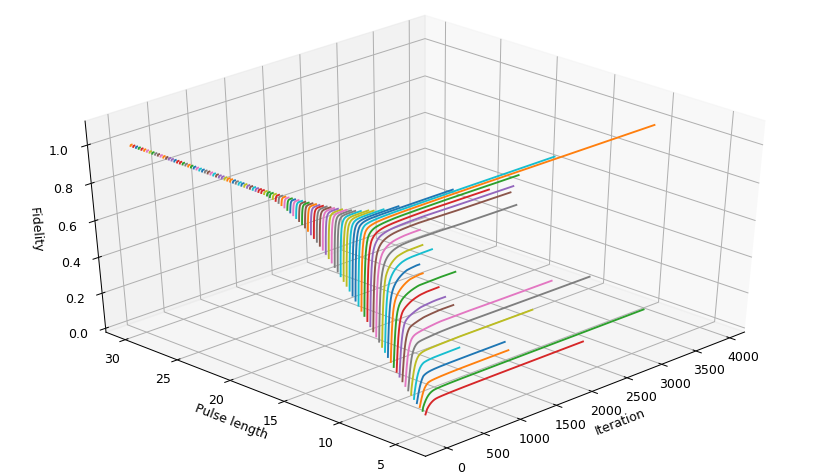
\includegraphics[width=\linewidth]{figs/3d-optim-ge.png}
    \caption{Caption}
    \label{fig:3d-optim-ge}
\end{figure}

\begin{figure}
    \centering
    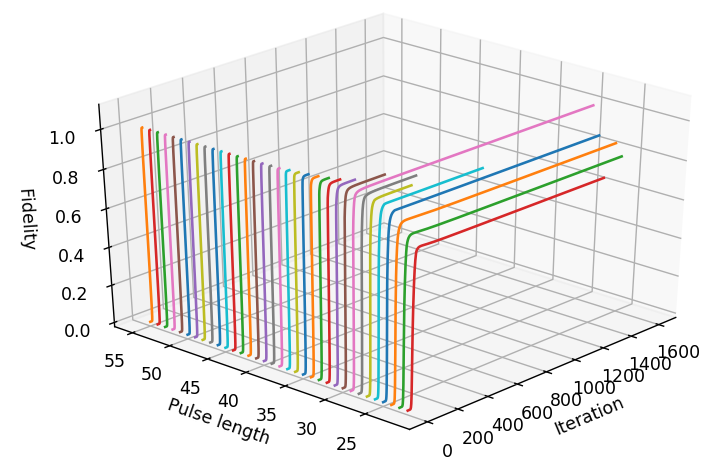
\includegraphics[width=0.7\linewidth]{figs/3d-optim-gf.png}
    \caption{Caption}
    \label{fig:3d-optim-gf}
\end{figure}

\tikzfig{figs/fidelity-length-ge}{Text}{fig:fidelity-length-ge}{15em}{15em}
\tikzfig{figs/fidelity-length-gf}{Text}{fig:fidelity-length-gf}{15em}{15em}

\tikzfig{figs/pulse_shape_4,25_Real}{Text}{fig:pulse_shape_4,25_Real}{\textwidth}{15em}
\tikzfig{figs/pulse_shape_4,25_Imag}{Text}{fig:pulse_shape_4,25_Real}{\textwidth}{15em}



\tikzfig{figs/pulse_shape_30,0_Real}{Text}{fig:pulse_shape_30,0_Real}{\textwidth}{15em}
\tikzfig{figs/pulse_shape_30,0_Imag}{Text}{fig:pulse_shape_30,0_Real}{\textwidth}{15em}


\tikzfig{figs/pulse_spectrum_30,0}{Text}{fig:fidelity-length}{25em}{15em}
\tikzfig{figs/pulse_spectrum_30,0}{Text}{fig:pulse_spectrum_30,0}{25em}{15em}

\begin{figure}
\centering
\foreach \n/\capn in {{4,25}/{4.25},{6,0}/{6.0},{8,0}/{8.0},{9,0}/{9.0},{10,0}/{10.0},{30,0}/{30.0}}{
	\subcaptionbox{Pulse length \capn{} ns}{
		\centering
		\setlength\figureheight{15em}
		\setlength\figurewidth{0.47\textwidth}
		\input{figs/pulse_spectrum_\n.tikz}
	}%
	\hfill
}
\caption{Time dynamics on the Bloch sphere for different lengths of optimised pulses.}
\label{fig:pulse_spectrum}
\end{figure}


\begin{figure}
\centering
\foreach \n/\capn in {{4,25}/{4.25},{6,0}/{6.0},{8,0}/{8.0},{9,0}/{9.0},{10,0}/{10.0},{30,0}/{30.0}}{
	\subcaptionbox{Pulse length \capn{} ns}{\includegraphics[width=0.3\linewidth]{figs/bloch_evolution_\n.png}}%
	\hfill
}
\caption{Time dynamics on the Bloch sphere for different lengths of optimised pulses.}
\label{fig:bloch_evolution}
\end{figure}

\section{0 to 2 transfer}

\begin{figure}
\centering
\foreach \n/\capn in {{22,0}/{22.0},{24,0}/{24.0},{26,0}/{26.0},{28,0}/{28.0},{29,0}/{29.0},{55,0}/{55.0}}{
	\subcaptionbox{Pulse length \capn{} ns}{
		\centering
		\setlength\figureheight{15em}
		\setlength\figurewidth{0.47\textwidth}
		\input{figs/pulse_spectrum_gf_\n.tikz}
	}%
	\hfill
}
\caption{Time dynamics on the Bloch sphere for different lengths of optimised pulses.}
\label{fig:pulse_spectrum}
\end{figure}


\begin{figure}
\centering
\foreach \n/\capn in {{22,0}/{22.0},{24,0}/{24.0},{26,0}/{26.0},{28,0}/{28.0},{29,0}/{29.0},{55,0}/{55.0}}{
	\subcaptionbox{Pulse length \capn{} ns}{\includegraphics[width=0.3\linewidth]{figs/bloch_evolution_gf_\n.png}}%
	\hfill
}
\caption{Time dynamics on the Bloch sphere for different lengths of optimised pulses.}
\label{fig:bloch_evolution}
\end{figure}

\end{document}
